\chapter{Future Work} \label{ch:future-work}
\markboth{Future Work}{}

Regarding the future, we believe that this thesis is only the starting point of an innovative approach towards a new paradigm for the democratization of IoT Edge Computing and the Internet of Things. Having introduced a high level architecture, our first objective is to continue the research and create the proper specifications for the entire architecture, including the components ,the described processes and proceed to the verification and validation of the proposed system. On top of that, there are various elements that are presented or mentioned in our work that merit more thorough research, namely in the areas of security, distributed systems and Internet of things.

We find that the following areas are ripe for research:
\begin{itemize}
    \item Required Resources estimation for a given container image
    \item Resources evaluation for a given Edge device
    \item A Filecoin light client ( “light” = It doesn’t need to download the entirety of the blockchain)
    \item A “Chinese” wall between containers and hostOS, keeping the good parts of the container technology while eliminating security issues between a hostile host and a trusted container or 
    vice-versa.
    \item Container intercommunication over a hostile environment
    Edge \& Central Arbitrator architecture

\end{itemize}

We envisage a system where various stakeholders can use established Edge Nodes devices to manage their IoT sensors and constrained devices, decoupling in essence the infrastructure owner and the end-user. Moreover, this model can be used in the cloud layer, where stakeholders will rent fully functional IoT platform systems (as opposed to services such as AWS where you rent cloud resources) to manage their IoT fleet.

\begin{figure}[h]
    \centering
    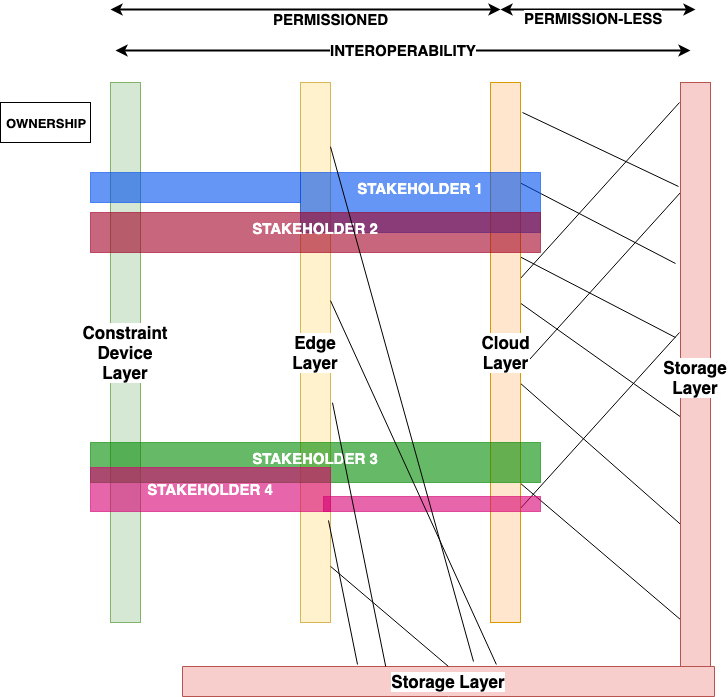
\includegraphics[width=0.9\textwidth]{images/layers_now_v2.png}
    \caption{The IoT reference architecture as a series of layers, partly decentralized }
    \label{fig:layers_now}
\end{figure}

In Figure \ref{fig:layers_now} we demonstrate the 4 distinct layers of the system, showcasing the subsystems that act in a permissioned \& trusted environment and the Storage Layer which does not. We also demonstrate the vertical slices of different stakeholders, where the overlap indicates that they are in fact participating in a contract. The different lines between the Cloud Layer and the Storage Layer illustrate that any stakeholder from the Cloud Layer can connect and store, in fact, to any stakeholder in the Storage Layer.
 
While the current implementation and architecture features a centralized system, we foresee that the breakthrough will be achieved in a fully decentralized system, where Edge \& Cloud nodes will be rented dynamically and the hand-over will be done almost seamlessly. Exploiting Distributed Ledger Technologies (such as the blockchain) we envisage a system where any stakeholder can participate and offer or demand Edge \& Cloud services. Moreover, this system will enable the participants to perform transactions of services and value without demanding trust amongst the parties and without requiring central authority to permit participation or to behave as an oversight authority. The envisaged future architecture is shown in Figure \ref{fig:layers_decent}.

\begin{figure}[h]
    \centering
    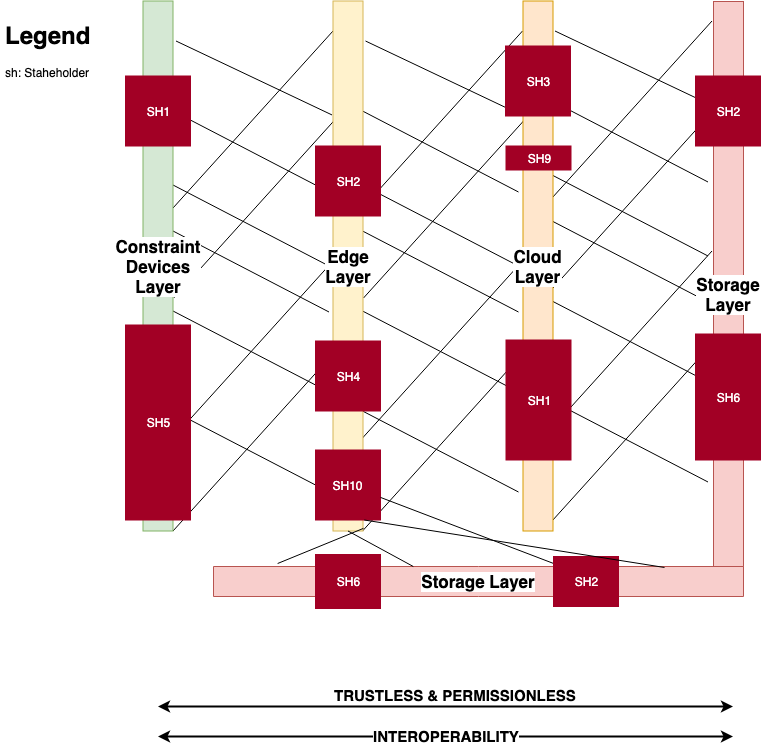
\includegraphics[width=0.9\textwidth]{images/layers_decentralized_v2.png}
    \caption{The IoT reference architecture as a series of decentralized networks that form it's layers}
    \label{fig:layers_decent}
\end{figure}


Figure \ref{fig:layers_decent} is similar to figure \ref{fig:layers_now} but features a completely decentralized model.

Each red box is the system that belongs to a different stakeholder, while the size of the boxes are proportional to the size of the infrastructure, qualitatively,

Each line models the Parent-Children relationship between subsystems of different layers. We demonstrate that \textit{any} constraint device can use \textit{any} edge device as a gateway and \textit{any} edge device can use \textit{any} cloud system as back-end. \textit{Any} is used in a qualitative manner as we are describing a dynamic market where demand \& offer will be determined by many different parameters. The devices, in any layer, have a set of parameters that forbid certain connections, the most prominent one being the connectivity protocol. It is apparent that a contraint device which exclusively supports Zigbee can not be managed by an IoT Edge that supports BLE (Blueetooth Low Energy) and LoRa.

We hope that our research will contribute towards the end goal of a decentralized IoT Edge computing System, where the interoperability will enable the democratization of the domain and the proliferation of IoT devices, by enabling any device to interface to any Edge or Cloud computing system. 
